% Original teaching figure; displayed coordinate windows are intentionally different.
\documentclass[tikz,border=3mm]{standalone}
\begin{document}
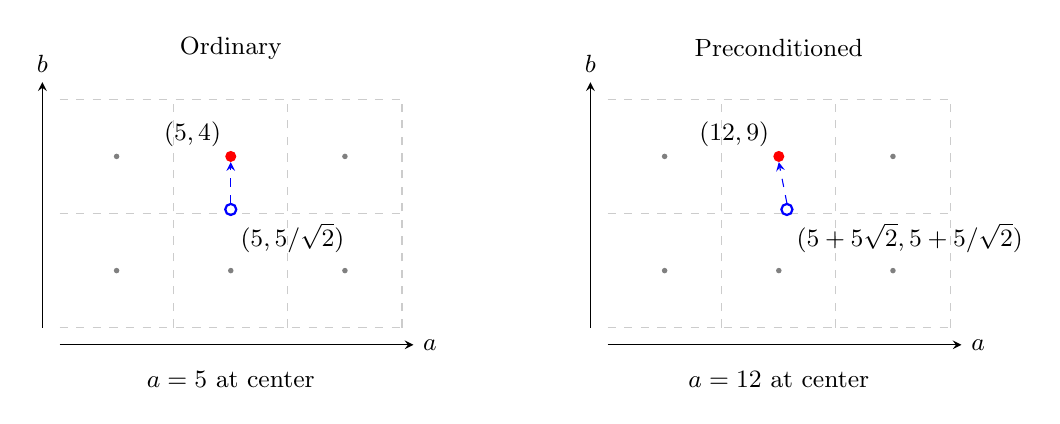
\begin{tikzpicture}[>=stealth,font=\small,x=1.45cm,y=1.45cm]
\foreach \offset/\base/\height/\title in {0/5/3/Ordinary,4.8/12/8/Preconditioned} {
\begin{scope}[shift={(\offset,0)}]
\foreach \s in {-1,0,1} {
\draw[gray!40,dashed] (\s+.5,-.5)--(\s+.5,1.5);
\draw[gray!40,dashed] (-1.5,\s+.5)--(1.5,\s+.5);
}
\foreach \x in {-1,0,1} \foreach \y in {0,1} \fill[gray] (\x,\y) circle (1pt);
\draw[->] (-1.5,-.65)--(1.6,-.65) node[right] {$a$};
\draw[->] (-1.65,-.5)--(-1.65,1.65) node[above] {$b$};
\node at (0,-.95) {$a=\base$ at center};
\node at (0,1.95) {\title};
\ifnum\base=5
\draw[blue,thick] (0,.535534) circle (2pt);
\draw[->,blue,dashed] (0,.59)--(0,.95);
\node[below right] at (0,.5) {$(5,5/\sqrt2)$};
\else
\draw[blue,thick] (.071068,.535534) circle (2pt);
\draw[->,blue,dashed] (.071068,.59)--(0,.95);
\node[below right] at (.071068,.5) {$(5+5\sqrt2,5+5/\sqrt2)$};
\fi
\fill[red] (0,1) circle (2pt);
\node[above left] at (0,1) {$(\base,\number\numexpr\height+1\relax)$};
\end{scope}
}
\end{tikzpicture}
\end{document}
